\documentclass[12pt,utf8]{beamer}
\setbeamercovered{transparent}
\usepackage[german]{babel}
\usepackage{color}
\usepackage{xcolor}
\usepackage{graphicx}
\usepackage{tikz}
\usepackage{../Latex_Template/beamerthemeFOSSAG}

\title{Linux Basics}
\subtitle{Das Terminal}

\author[J.-M. Lenk, C. Parnitzke, Y. Bungers, A. Becker]{Jan-Marius Lenk, Christoph Parnitzke, Yannick Bungers, Alexander Becker}
\institute[FOSS AG]{Free and Open Source Software AG\\ Fakultät für Informatik}

\date{\today}

\begin{document}

\titlepage

\begin{frame}
\frametitle{Inhaltsverzeichnis}
\begin{itemize}
	\item Einleitung
	\item Arbeiten mit Ordnern, Dateien und Archiven
	\item Systemverwaltung
\end{itemize}
\end{frame}

\section{Einleitung}
\begin{frame}
\frametitle{Unix Philosophie}
\begin{figure}

\includegraphics[scale=0.15]{res/tuX_tu.png}
\end{figure}
\begin{itemize}
	\item Philosophie besteht aus drei Punkten:
	\begin{enumerate}
		\item Schreibe Programme, die nur eine Sache tun und dies erfolgreich
		\item Schreibe Programme, die Kolaboration ermöglichen
		\item Schreibe Programme, die mit Text arbeiten, denn dies ist universell
	\end{enumerate}
\end{itemize}
%\footnote{https://upload.wikimedia.org/wikipedia/commons/a/af/Tux.png}
\end{frame}

\section{Arbeiten mit Ordnern, Dateien und Archiven}
\subsection{Ordner}
\begin{frame}
	\frametitle{\textcolor{highlight}{l}i\textcolor{highlight}{s}t}
	\framesubtitle{Ein kleines Licht in der Dunkelheit}
	\begin{itemize}
		\item Listet alle Ordner und Dateien in Verzeichnis auf
		\item Mögliche Optionen:
		\begin{itemize}[<+->]
			\item \texttt{-a}  (all) inkl. versteckter Verzeichnisse
			\item \texttt{-hl}  (human readable / long listing format) inkl. Rechte, Besitzer, Größe, etc.
		\end{itemize}
	\end{itemize}
\end{frame}

\begin{frame}
	\frametitle{\textcolor{highlight}{c}hange \textcolor{highlight}{d}irectory}
	\framesubtitle{Die kleine Form der Teleportation}
	\texttt{cd} ermöglicht das Navigieren durch das Dateisystem
	\begin{itemize}
		\item Wechsel in Parent-Directory mit \texttt{cd ..}
		\item Wechsel in Home-Directory mit \texttt{cd} ($\sim$)
	\end{itemize}
\end{frame}

\begin{frame}
\frametitle{\textcolor{highlight}{c}o\textcolor{highlight}{p}y $\&$ \textcolor{highlight}{m}o\textcolor{highlight}{v}e}
\framesubtitle{Die Kunst des Klonens und Umbenennens}
\begin{itemize}
	\item \texttt{mv PATH1 PATH2} (Verschieben von Dateien/Ordnern)
	\item \texttt{cp PATH1 PATH2} (Kopieren von Dateien)
	\begin{itemize}
		\item -r ermöglicht kopieren von Ordnern
	\end{itemize}
\end{itemize}
\end{frame}

\begin{frame}
\frametitle{\textcolor{highlight}{m}a\textcolor{highlight}{k}e \textcolor{highlight}{dir}ectory}
\framesubtitle{Verzeichnisse erschaffen}
\texttt{mkdir} erstellt Ordner auf dem Rechner
\begin{itemize}
	\item \texttt{mkdir PATH}
	\item \texttt{-p} erstellt alle Ordner auf dem Pfad, die noch nicht existieren
\end{itemize}
\end{frame}

\begin{frame}
\frametitle{\textcolor{highlight}{r}e\textcolor{highlight}{m}ove}
\framesubtitle{Flutsch! Und weg!}
\begin{itemize}
	\item \texttt{rm [OPTION] FILE}
	\begin{itemize}[<+->]
		\item \texttt{-r} ermöglicht das Löchen von Ordnern
	\end{itemize}
\end{itemize}
\end{frame}

\begin{frame}
	\frametitle{find}
	\texttt{find} sucht Dateien im aktuellen Ordner und in Unterordnern
	\begin{itemize}
		\item \texttt{find -name FILE}
	\end{itemize}
\end{frame}

\subsection{Archive}
\begin{frame}
\frametitle{\textcolor{highlight}{t}ape \textcolor{highlight}{ar}chiver}
\framesubtitle{Archivieren}
Zum entpacken von Archiven wie \texttt{.tar}, \texttt{.tar.gz}, \texttt{.zip}, etc. 
\begin{itemize}
	\item \texttt{tar -czvf ARCHIVE\_PATH PATH\_FILES}\\(Verpacken)
	\item \texttt{tar -xzvf ARCHIVE\_PATH}\\(Entpacken)
\end{itemize}
\end{frame}

\begin{frame}
\frametitle{\Large{\textcolor{highlight}{g}lobally search a \textcolor{highlight}{r}egular \textcolor{highlight}{e}xpression and \textcolor{highlight}{p}rint}}
\framesubtitle{Gonna catch em' Strings}
\texttt{grep} ermöglicht die Suche in einer Eingabe
\begin{itemize}
	\item \texttt{-i} ignoriert Groß- und Kleinschreibung bei der Suche
\end{itemize}
\end{frame}

\begin{frame}
\frametitle{man page}
\framesubtitle{Wenn man mal nicht weiter weiß}
Anleitungen (Manuals) zu den installierten Paketen lassen sich mit \texttt{man} betrachten.
\begin{itemize}
	\item man COMMAND
\end{itemize}
\end{frame}

\begin{frame}
\frametitle{\textcolor{highlight}{t}ape \textcolor{highlight}{ar}chiver}
\framesubtitle{Archivieren}
\begin{itemize}[<+->]
\item {\scriptsize \texttt{-c} (create) erzeugt neues Archiv}
\item {\scriptsize \texttt{-x} (extract) extrahieren einer Datei}
\item {\scriptsize \texttt{-v} (verbose) Fortschritt auflisten}
\item {\scriptsize \texttt{-z} (gzip format) komprimieren als \texttt{.gz}, etc.}
\item {\scriptsize \texttt{-f} erzeugt beim Entpacken einen Ordner mit Namen von Archiv}
\end{itemize}
\end{frame}

\begin{frame}
\frametitle{\Large Dateien betrachten und bearbeiten}
\begin{itemize}
	\item \texttt{cat FILE} - Ausgabe einer Datei
	\item \texttt{less FILE} - Betrachten einer Datei
	\item \texttt{nano FILE} - Bearbeiten einer Datei
\end{itemize}
\end{frame}

\subsection{Dateien}
\begin{frame}
	\centering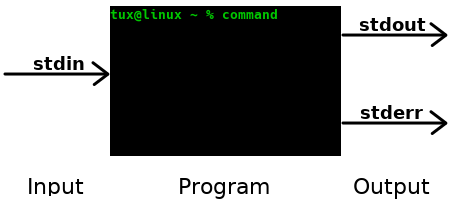
\includegraphics[scale=0.65]{res/IOE}
\end{frame}

\begin{frame}
	\Huge\centering{$|$~~~$>$}
\end{frame}

\begin{frame}
\Huge\centering{\&}
\end{frame}

\section{Systemverwaltung}
\subsection{Prozesse verwalten}
\begin{frame}
\frametitle{\textcolor{highlight}{h}isham \textcolor{highlight}{t}able \textcolor{highlight}{o}f \textcolor{highlight}{p}rocesses}
\framesubtitle{interaktiver Prozessmanager}
\begin{itemize}
	\item \texttt{\textcolor{red}{t}able \textcolor{red}{o}f \textcolor{red}{p}rocesses} (bereits installtiert)
	\item \texttt{htop} (muss installiert werden)
	\begin{itemize}[<+->]
		\item {\scriptsize Übersicht über alle Prozesse und verbrauchte Ressourcen}
		\item {\scriptsize deutlich leichtere Bedienung und bessere Übersicht}
		\item {\scriptsize bietet mehr Interaktionen}
	\end{itemize}
\end{itemize}
\end{frame}

\subsection{Paketverwaltung}
\begin{frame}
	\frametitle{\textcolor{highlight}{s}uper \textcolor{highlight}{u}ser \textcolor{highlight}{do}}
	\framesubtitle{Mit großer Macht kommt große Verantwortung}
	\texttt{sudo} führt einen Befehl mit administrativer Berechtigung aus
	\begin{itemize}
		\item \texttt{sudo COMMAND}
	\end{itemize}
\end{frame}

\begin{frame}
	\frametitle{apt}
	Mit \texttt{apt} lassen sich Pakete installieren und deinstallieren
	\begin{itemize}
		\item \texttt{sudo apt install PACKAGE}
		\item \texttt{sudo apt update}
		\item \texttt{sudo apt upgrade / dist-upgrade}
		\item \texttt{sudo apt remove PACKAGE}
		\item \texttt{sudo apt search PACKAGE}
	\end{itemize}
\end{frame}

\subsection{Herunterfahren und Neustarten}
\begin{frame}
\frametitle{poweroff und reboot}
\framesubtitle{Wenn man mal das real life genießen will}
\begin{itemize}
	\item \texttt{poweroff} (Herunterfahren des Systems)
	\item \texttt{reboot} (Neustart des Systems)
\end{itemize}
\end{frame}

\subsection{Übersicht}
\begin{frame}
\frametitle{\LARGE Übersicht}
%framesubtitle{Alle Befehle auf einen Blick}
\small
\begin{minipage}{0.48\linewidth}
	\begin{itemize}
		\item \texttt{ls} - Dateien auflisten
		\item \texttt{cp} - Datei kopieren
		\item \texttt{mv} - Datei verschieben
		\item \texttt{mkdir} - Ordner erstellen
		\item \texttt{rm} - Dateien löschen
		\item \texttt{find} - Dateien suchen
		\item \texttt{tar} - Archive verarbeiten
		\item \texttt{grep} - Text durchsuchen
		\item \texttt{man} - Anleitung anzeigen
	\end{itemize}
\end{minipage}
\begin{minipage}{0.48\linewidth}
	\begin{itemize}
		\item \texttt{less} - Datei betrachten
		\item \texttt{nano} - Texteditor
		\item \texttt{top/htop} - Prozessverwaltung
		\item \texttt{sudo} - Befehl als Root ausführen
		\item \texttt{apt} - Paketverwaltung
		\item \texttt{poweroff} - Herunterfahren
		\item \texttt{reboot} - Neustarten
	\end{itemize}
\end{minipage}

\end{frame}

\end{document}
